\documentclass[ letterpaper, titlepage, fleqn]{article}

\usepackage[utf8]{inputenc}
\usepackage[slovene]{babel}
\usepackage[margin=60px]{geometry}
\usepackage{amsmath}
\usepackage{amssymb}
\usepackage{enumerate}
\usepackage{graphicx}
\usepackage{mathrsfs}
\setlength\parindent{0pt}

\begin{document}

\title{$\sigma$-irregularity vs. total $\sigma$-irregularity}
\author{Nejc Ševerkar \& Anja Trobec}
\date{\today}
\maketitle
\pagebreak

\thispagestyle{empty}
\tableofcontents
\pagebreak

\section{Uvod}

V projektni nalogi se bova ukvarjala z meritvijo iregularnosti enostavnih neusmerjenih grafov z
dvema na videz podobnima metodama, {\em $\sigma$-irregularity} in {\em total $\sigma$-irregularity},
definiranima kot 
$$
\sigma(G) = \sum_{(u, v) \in E(G)}(d_u - d_v)^2 
\quad \text{in} \quad
\sigma_t(G) = \sum_{(u, v) \in V(G)}(d_u - d_v)^2
$$
Cilj naloge je maksimizacija razmerja 
$$\sigma_r(G) = \frac{\sigma_t(G)}{\sigma(G)}$$
pri danem redu grafa $n \in \mathbb{N}$.
Ker nas komponentno regularni grafi, za katere to razmerje ni definirano,
torej v primeru $\sigma(G) = 0$, ne zanimajo, definiramo $\sigma_r(G) = 0$.
\\\\
V nadaljevanju bomo zaradi preprostosti prostor grafov na $n$ vozliščih označevali z $\mathscr{G}_n$.
\\\\
Najina glavna naloga je torej poiskati maksimalno razmerje $\sigma_r(G)$ za $G \in \mathscr{G}_n$ in graf, 
pri katerem je razmerje doseženo. To nama bo v pomoč pri preverjanju naslednjih dveh hipotez.
\begin{itemize}
\item[(i)] Stopnja naraščanja optimalnega $\sigma_r$ razmerja je $O(n^2)$.
\item[(ii)] V optimalnem grafu se stopnje vseh sosednjih vozlišč razlikujejo za največ 1.
\end{itemize}
Prvo hipotezo bova preverila s polinomsko aproksimacijo $\sigma_r$ naraščanja, 
ki bo izvedena s pomočjo metode najmanjših kvadratov.
Drugo pa bova preverila s številom parov vozlišč, ki ne ustrezajo hipotezi in izračunom njihovih stopenjskih razlik.

Proti koncu bova povedala še nekaj splošnega o distribuciji stopenj vozlišč v optimalno dobljenih grafih.

\section{Osnovna Teorija}

\subsection{Maksimalna Stopnja Naraščanja}
Ker bomo za analizo in primerjavo potrebovali stopnjo naraščanja
zaporedja $(\max_{G_n \in \mathscr{G}_n} \sigma_r(G_n))_n$ bo koristno izračunati zgornjo mejo.

Poskušajmo maksimizirati vrednost $\sigma_t(G)$ za dani graf $G$.
Po premisleku se lahko prepričamo, da bo za graf $G \in \mathscr{G}_n$ največja vrednost $\sigma_t(G)$ dosežena, če
bodo vsa vozlišča stopenj $n - 1$ in $0$, saj bo tako kvadratična razlika med njimi največja.
Zanima nas torej število vozlišč s stopnjo $n$, $x$, ki maksimizira funkcijo
$f(x) = x (n - x)$, saj ta predstavlja število kombinacij parov vozlišč s stopnjo $n - 1$ in $0$.
Z odvajanjem poiščemo maksimum, ki je dosežen pri $n / 2$, zato velja
$$
\sigma_r(G) = \frac{\sigma_t(G)}{\sigma(G)} 
\leq \sigma_t(G) \leq \frac{n}{2} \frac{n}{2} (n - 1)^2 
= O(n^4).
$$
Sledi, da je zgornja meja naraščanja $O(n^4)$.

\subsection{Nepovezani Grafi}
Ker sva opazila, da družina nepovezanih grafov doseže maksimalno stopnjo naraščanja,
se lahko po konstrukciji družine takšnih grafov $G_n$ za $\forall n \in \mathbb{N}$
osredotočimo samo na povezane grafe.

Konstrukcija grafov $G_n$, za katere ima zaporedje  $(\max_{G_n \in \mathscr{G}_n} \sigma_r(G_n))_n$  stopnjo 
naraščanja $O(n^4)$ je sledeča.
Vzamemo $n / 2$ vozlišč in iz njih konstruiramo poln graf
medtem, ko v preostalih $n /2$ vozliščih povežemo 3 vozlišča z dvema povezavama.
Po kratkem premisleku lahko formuliramo naslednjo neenakost.
$$\sigma_r(G_{2n}) = \frac{\sigma_t(G_{2n})}{\sigma(G_{2n})} =  \frac{\sigma_t(G_{2n})}{2}  > \frac{(n - 3) n (n - 1)^2}{2} = \Theta(n^4)$$.
\\
S tem sva zaključila preučevanje nepovezanih grafov.

\section{Ideja Iskanja Optimalnih Grafov}
Problem bova reševala v Pythonu in si občasno pomagala s knjižnjico Networkx,  
s katero bodo grafično predstavljeni grafi.

\subsection{Metahevristike}
Za optimalno vrednost $\sigma_r$ na grafih reda $n$ bi morala testirati vse neizomorfne
grafe tega reda, kar pa bi zahtevalo testiranje vseh grafov $G \in \mathscr{G}_n$, 
katerih pa je $\Omega(2^{\binom{n}{2}})$. Če upoštevamo, da izračun $\sigma_r(G)$ 
zahteva $\Omega(n^2)$ operacij, dobimo skupno časovno zahtevnost $\Omega(n^2 2^{\binom{n}{2}})$.
Očitno ta zahtevnost predstavlja problem že za grafe reda $10$, 
torej bova morala poiskati alternativni pristop v obliki metahevrističnih algoritmov.
Ideja bo torej sistematično postopati po prostoru povezanih enostavnih grafov reda $n$ in 
tako iskati aproksimacijo grafa $G$, ki maksimizira vrednost $\sigma_r$ na tem prostoru.
Za učinkovito delovanje teh procesov pa potrebujemo definirati ustrezno topologijo 
na prostoru, torej podati pojem bližine, saj jo zahteva večina hevrističnih algoritmov.
To bova naredila med drugim tudi z zaporednim dodajanjem ali odstranjevanjem naključnih povezav v 
danem grafu, pri čimer morava paziti, da ohranjava povezanost grafa. 
Torej z drugimi besedami ne odstraniva mostov.
\\\\
Za te namene sva napisala knjižnjico, ki poda podporo za izbiro teh povezav
in splošno generiranje naključnih povezanih grafov, skupaj še z nekaterimi splošnimi orodji.

\subsection{Simulated Annealing}
Eden od algoritmov, ki naj bi rešil ta problem je {\em Simulated Annealing}, 
katerega implementacija je končana.
Algoritem je uporabljen za iskanje vseh optimalnih grafov v nadaljevanju naloge in parametriziran
s skupino parametrov, ki bo opisana kasneje.

\section{Reševanje Problema}

\subsection{Majhni grafi}
Za majhne grafe sva našla že generirane povezane neizomorfne grafe do stopnje 9 in poiskala vrednosti 
$$(M_n)_{n} = (\max_{G_n \in \mathscr{G}_n} \sigma_r(G_n))_{n=2}^9,$$
ki so zapisane v naslednji tabeli.

\begin{center}
    \begin{tabular}{ l | c }
      $n$ & $M_n$ \\ \hline
      2 & 0 \\ 
      3 & 1 \\ 
      4 & 3 \\ 
      5 & 3 \\ 
      6 & 5 \\ 
      7 & 13 \\ 
      8 & 19 \\ 
      9 & 14.5 \\ 
    \end{tabular}
\end{center}

Grafov na višjem številu vozlišč je preveč za posamično analizo, torej
se lotimo implementacije {\em Simulated Annealing} algoritma.

\subsection{Večji grafi}

Med večjimi grafi bomo optimume iskali s pomočjo algoritma SA ({\em Simulated Annealing}). 
Ta prejme 3 pomembne argumente: število vozlišč, število simulacij in definicijo okolice grafa.
Okolice so lahko poljubne in se delijo na lokalne in globalne.
Lokalne okolice spreminjajo graf po povezavah, globalne pa
konstruirajo nov graf, ki ima morda kakšne podobne karakteristike kot prejšnji.
\\\\
Izkazalo se je, da za velike grafe aplikacija lokalnih okolic ni dovolj. Zato
sva iskanje izvedla v dveh delih. Prvi del je klicanje SA na globalni okolici, nakar
pa še na lokalni, saj ta naredi na tem male optimizacije, ki jih globalne spremembe 
niso bile zmožne doseči.
Lokalno izboljšavanje nastopi v obliki minimizacije $\sigma(G)$ z osredotočanjem na
povezave, kjer je razlika med $d_G(u)$ in $d_G(v)$ za neka $uv \in E(G)$ največja.
\\\\
Po nekaj testih je začela biti očitna struktura optimalnih grafov in sicer
njihova oblika je sestavljena iz dveh delov. V prvem nastopa polni podgraf, 
na drugem pa so povezave redke in je zato podgraf blizu drevesu, kot lahko 
vidimo na spodnjih slikah grafov na 30, 40 in 50 vozliščih. \\
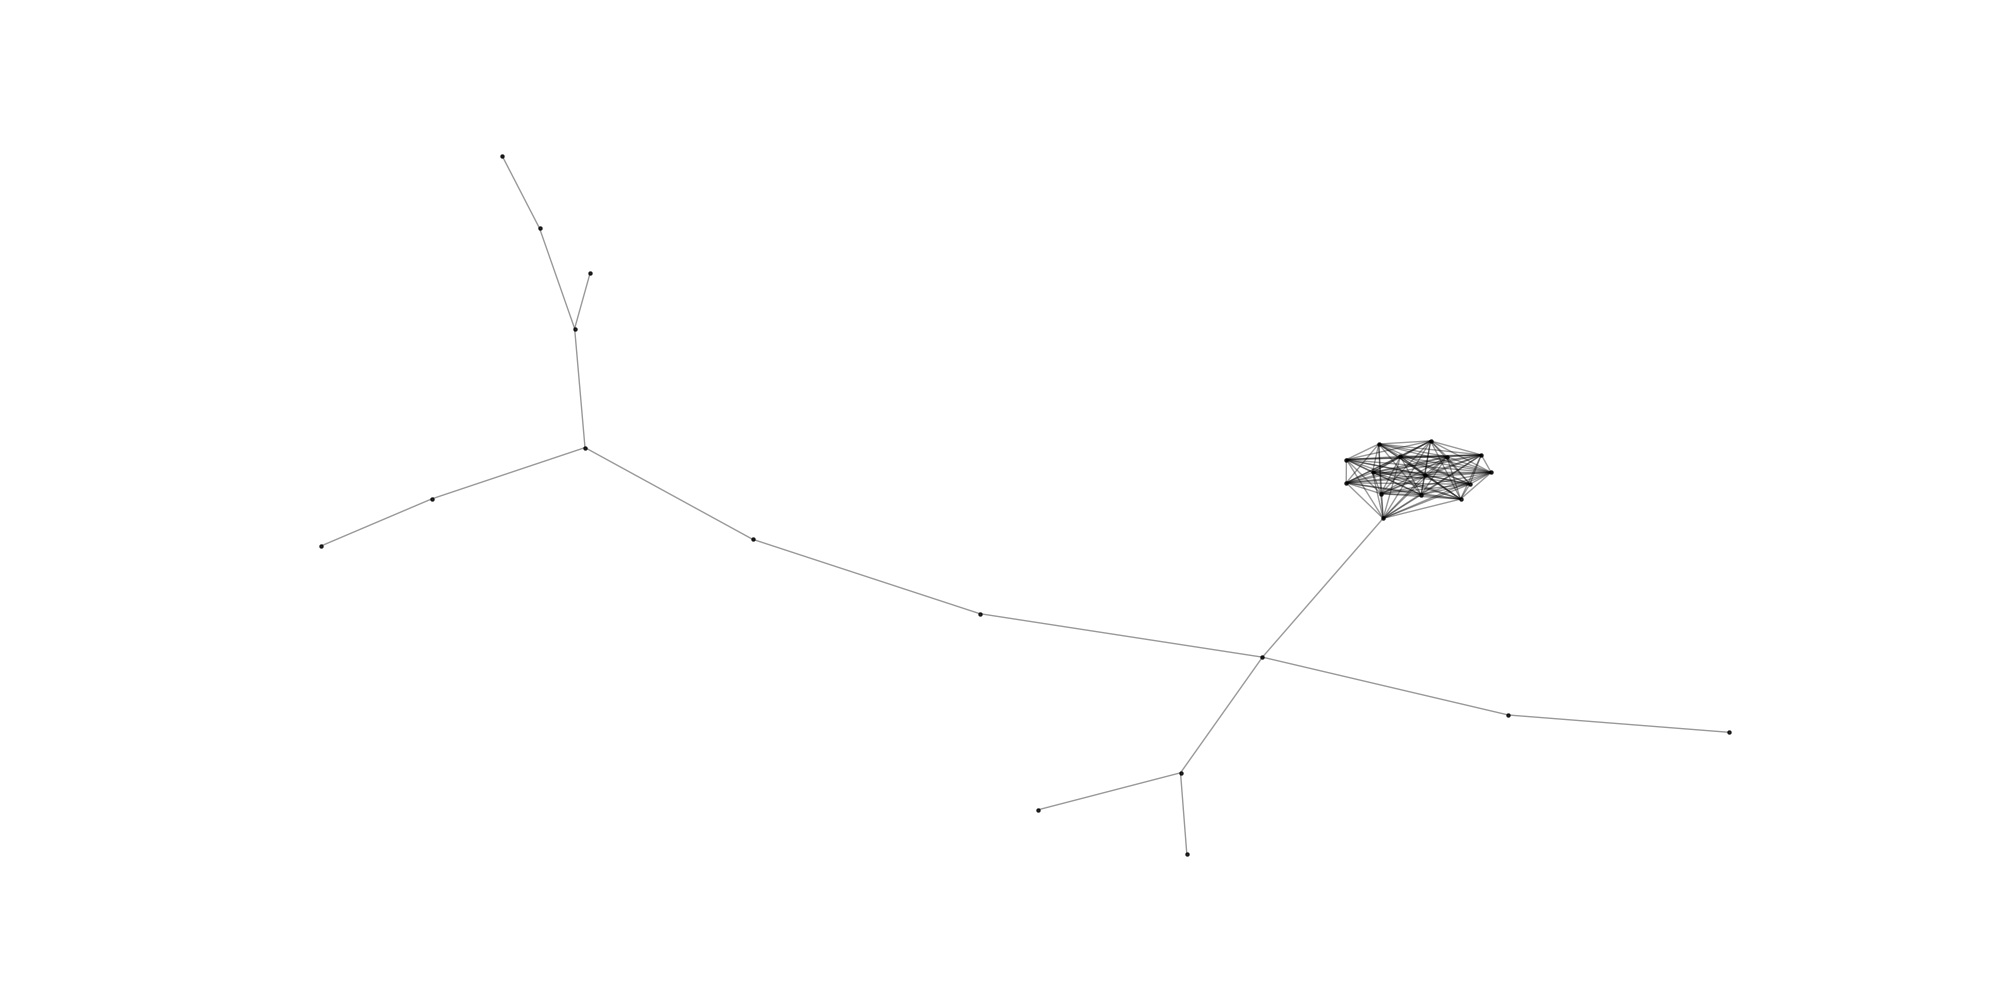
\includegraphics[width=8cm, height=5cm]{graphics/opt_sample_30.png}  
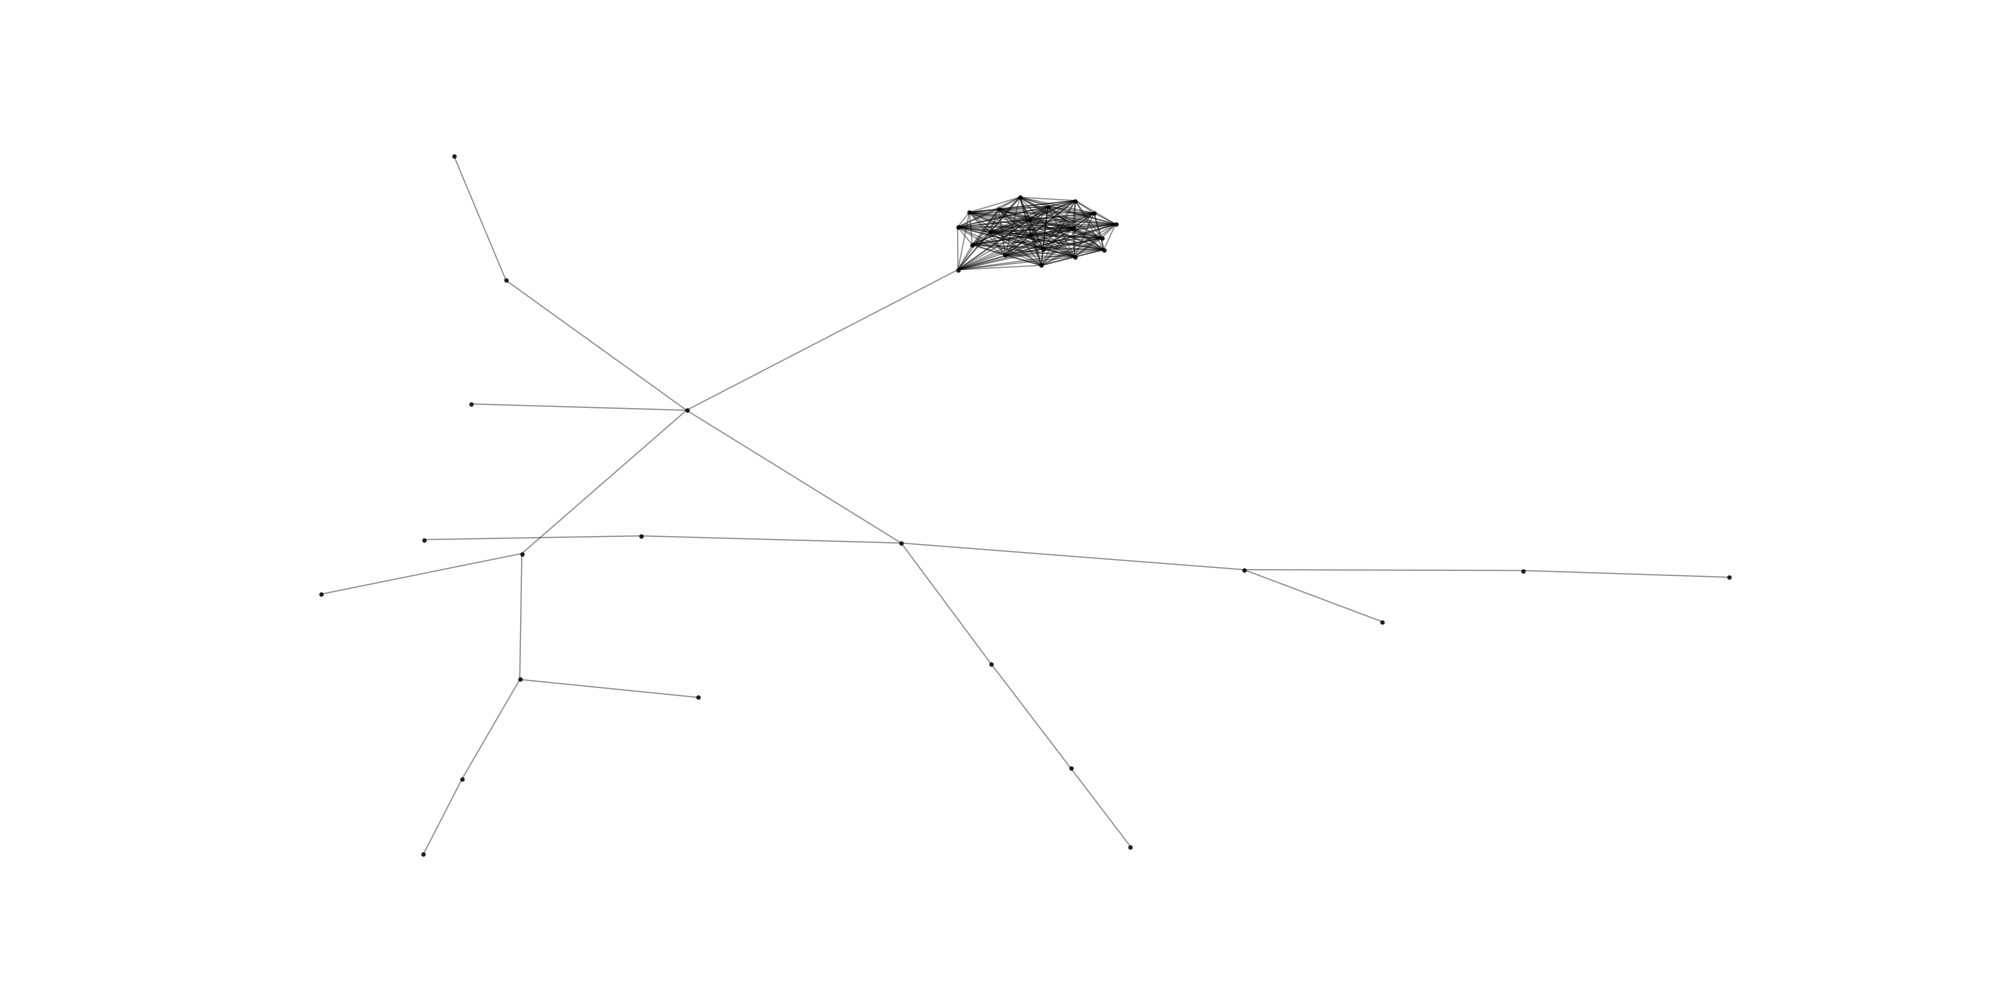
\includegraphics[width=8cm, height=5cm]{graphics/opt_sample_40.png}  \\
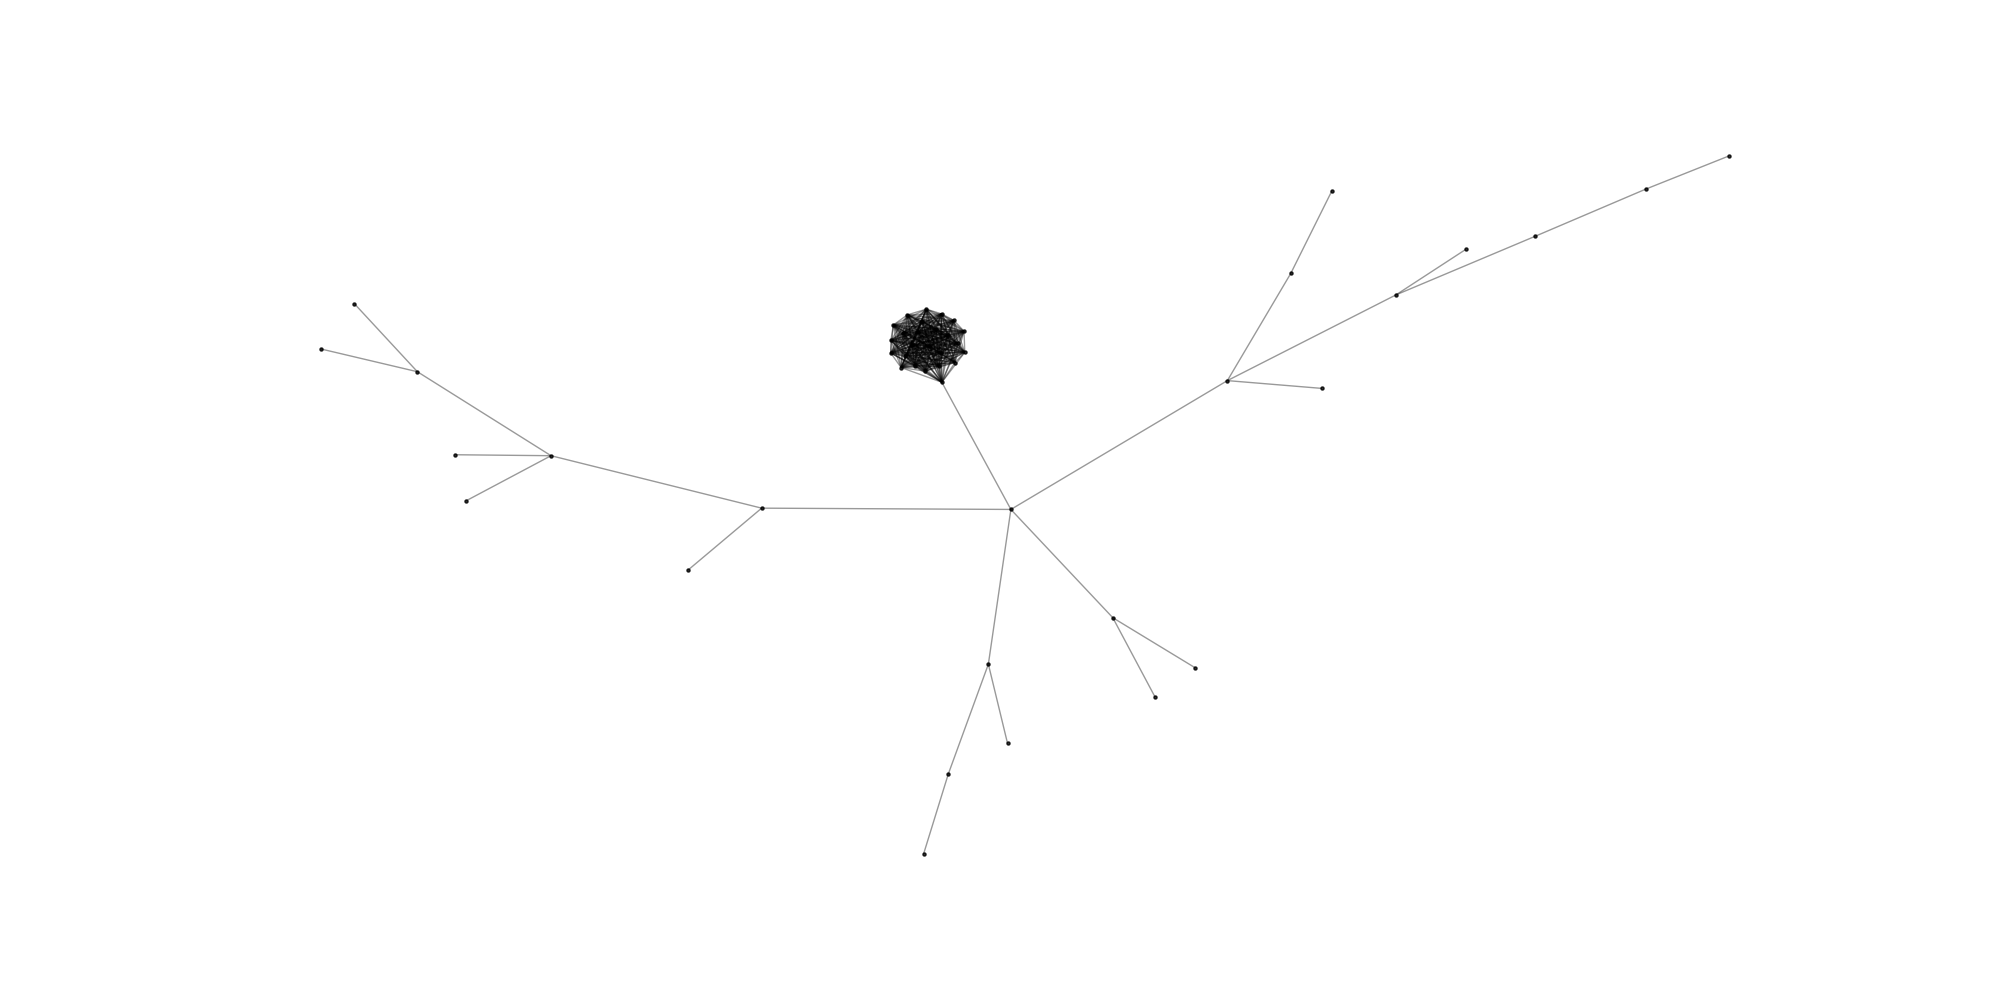
\includegraphics[width=\textwidth, height=5cm]{graphics/opt_sample_50.png} \\
Ta sestava je primerna, saj razlike med polnim grafom in redkim prispevajo 
k vrednosti $\sigma_t$, medtem ko vrednost $\sigma$ ostaja enaka, saj so v obeh
delih grafa sosednje povezave podobnih stopenj. To je skoraj res, a naletimo na posebno povezavo,
ki je prisotna v teh grafih in to je most med polnim in praznim podgrafom. Brez te povezave
bi imeli stopnjo naraščanja $O(n^4)$, a njena prisotnost znatno povišuje vrednost $\sigma$.
\\\\
Naš problem se po tej analizi prevede v to, kako 'zvezno', torej s čim manjšo razliko stopenj sosednih povezav, 
povezati poln podgraf z redkim. 
Za to potrebujemo veliko vozlišč, ki bodo poskrbeli za 'zvezno' pot med tima podgrafoma,  
a jih hkrati potrebujemo malo povezane, da maksimizirajo $\sigma_t$ vrednost, saj se ta primerja
z nastalim polnim grafom. Problem nam torej predstavljata tudi spodbijajoči optimizaciji $\sigma$ ter $\sigma_t$.
\\\\
V nadaljevanju si bomo pogledali katero optimizacijo favorizirajo optimalni grafi.

\subsection{Kvadratična stopnja naraščanja}
Preveriti morava, če je stopnja narašanja zaporedja
$(\max_{G_n \in \mathscr{G}_n} \sigma_r(G_n))_n$, za $n \in \mathbb{N}$
res $O(n^2)$. Tedaj pa poiskati ustrezno konstanto $c \in \mathbb{R}$, ki 
se naraščanju najbolj prilega.
\\\\
Predpostavimo, da smo optimum izračunali za $n$ grafov in označimo 
$$X(n, p) = (1^p, 2^p, \dots, n^p)^T \quad \text{in}\quad a = (a_1, a_2, \dots, a_n)^T$$
vektorja v $\mathbb{R}^{n}$, kjer $a_i$ predstavlja
dobljeni optimalni $\sigma_r(G_i)$ za graf $G_i \in \mathscr{G}_i$.
Problem pri danem $p \in \mathbb{R}^{+}$ zahteva rešitev linearnega sistema 
$$X(n, p)c = a.$$
Ta sistem seveda ne bo rešljiv, iskanja aproksimacije pa se bomo
lotili z metodo najmanjših kvadratov, torej minimum $2$-norme
razlike obeh strani bo dosežen pri
$$c = \frac{\langle a, X(n, p)\rangle}{||X(n, p)||_{2}^2}.$$

Najboljšo aproksimacijo naraščanja $\sigma_r$ bomo poiskali 
z diskretizacijo $D \subset [0, 4]$ in za $\forall p \in D$ 
izračunali prej definirani $c$, na koncu pa izbrali tisto kombinacijo
$(c, p)$, za katero je $||cX(n, p) - a||_{2}$ najmanjši.
\\\\
Tako dobimo po testiranju na vozliščih od $3$ do $700$ naslednji graf.\\
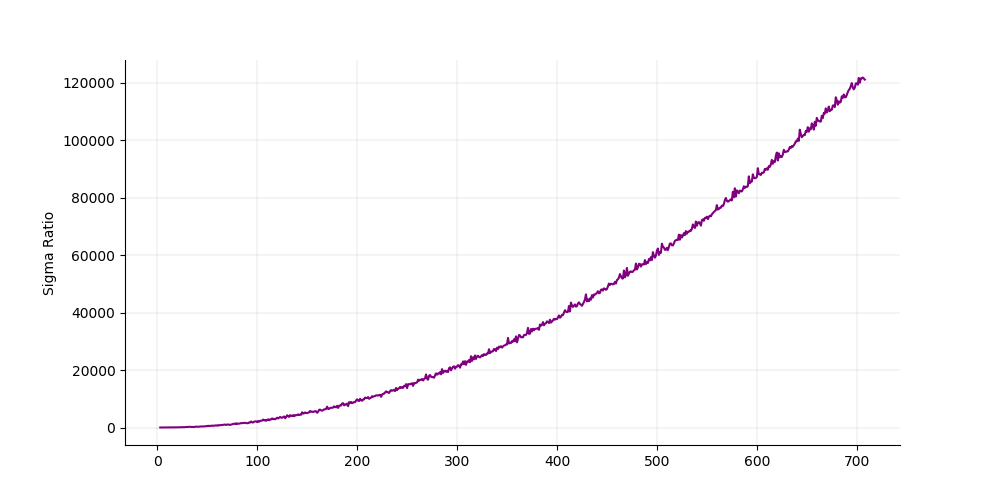
\includegraphics[width=\textwidth, height=8cm]{graphics/sigma_opts.png} \\
Po prej opisani metodi dobimo par $(c, p)$, za katerega $cn^p$ najbolje opisuje
$\sigma_r$ naraščanje. Ta par je izračunan kot $(0.1932, 2.0360)$ in
njegova aproksimacija naraščanja je prikazana na naslednjem grafu.\\
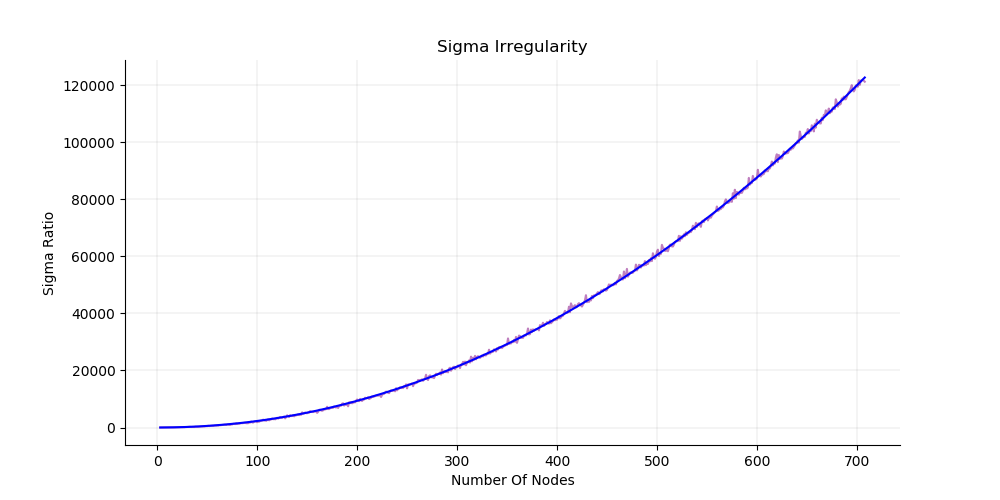
\includegraphics[width=\textwidth, height=8cm]{graphics/sigma_opts_aproximation.png}\\
Rezultati testiranja močno implicirajo kvadratično naraščanje zaporedja 
$(\max_{G_n \in \mathscr{G}_n} \sigma_r(G_n))_n$, saj pri večjih vzorcih varianca opazno pada,
hkrati pa se najboljša polinomska aproksimacija rasti približuje $n \to n^2$.
\pagebreak

\subsection{Hipoteza o stopnjah vozlišč}
Hipotezo, ki pravi, da so vsa sosednja vozlišča stopnje, ki se razlikuje za največ 1, bova testirala
z izračunom števila parov vozlišč, ki nimajo ustrezne razlike stopenj in seštela še vse njihove razlike.
Rezultati, skupaj z linearno aproksimacijo, so opisani na naslednjem grafu.\\
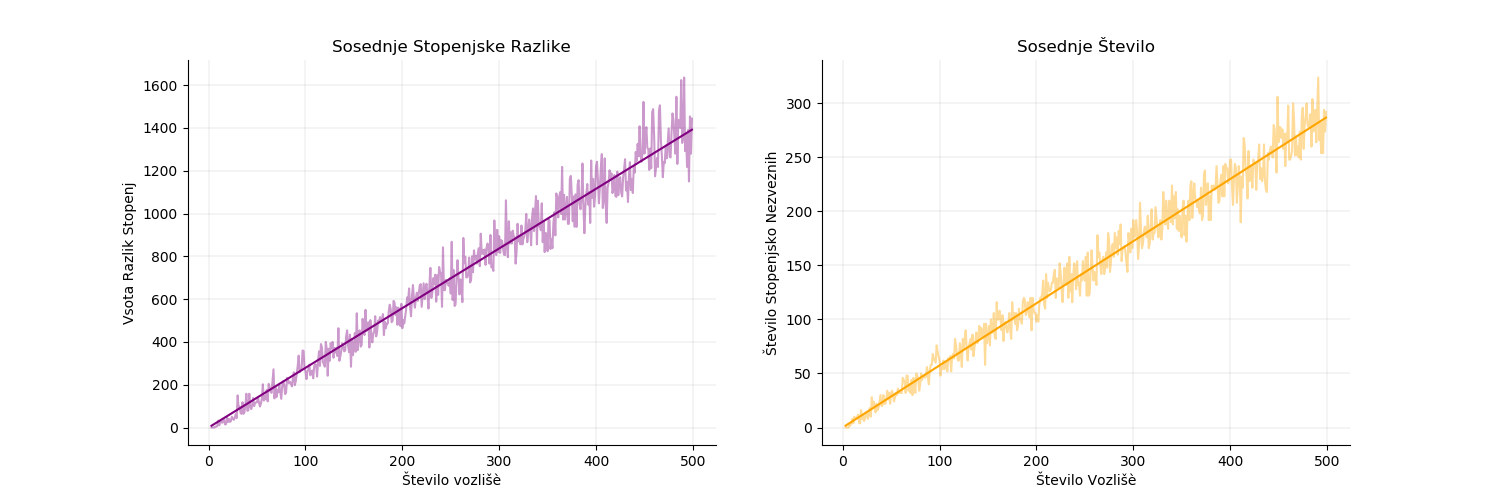
\includegraphics[width=\textwidth, height=6cm]{graphics/degree_difference_linear_aproximation.png}\\
Naraščanje je predvsem linearno in sicer sta najboljši linearni aproksiciji koeficientov enaki
$2.7895$ in $0.5749$, glede na horizontalno zaporedje slik.
\\\\
Na levem grafu vidimo, da je vsota stopenj vozišč majhna, saj je povprečno njena vrednost
le trikratnik števila vozlišč, torej se povprečno vozlišči na razliki stopenj večji od $1$ razlikujeta v stopnji za $3$, 
kot tudi namiguje koeficient.\\
Na desnem grafu takoj opazimo, da je naraščanje števila parov vozlišč, ki ne ustrezajo pogoju
zelo majhno, saj narašča počasneje kot stopnja vozlišč, čeprav je njeno potencialno naraščanje
$\binom{n}{2}$. 
Seveda je rezultat smiseln, saj poskušamo minimizirati $\sigma$ vrednost, katera pa narašča
skupaj z naraščanjem razlik stopenj sosednih vozlišč. 
\\\\
Vrnimo se nazaj na problem optimalnega povezanja polnega podgrafa s praznim. 
Sva mnenja, da so rezultati pozitivna indikacija na to, da se ta pot naravno formira na način, 
ki favorizira minimizacijo $\sigma$ vrednosti napram maksimizacije $\sigma_t$ vrednosti.
Torej grafi poskušajo poskrbeti za zvezni prehod iz polnega podgrafa k redkemu in za to 
žrtvujejo nekaj vozlišč, kar pa se na koncu pozna pri majhnih razlikah stopenj.

\subsection{Distribucija stopenj vozlišč}
Ideja bo prikazati minimalne in povprečne stopnje vozlišč pri danem optimalnem grafu na $n$ vozliščih.
Spodaj je prikazan graf, ki prikazuje prej povedano. \\
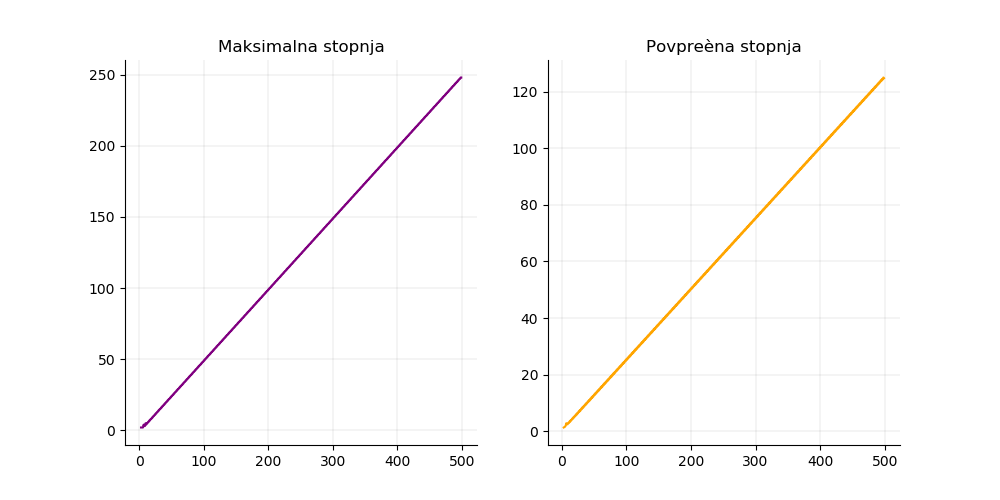
\includegraphics[width=\textwidth, height=6cm]{graphics/degree_distribution.png}\\
Iz slike je razvidno izredno linearno naraščanje maksimalne stopnje vozlišč in sicer za točni faktor $\frac{1}{2}$,
kar nas spomni na obliko optimalnih grafov, kateri imajo poln podgraf, vpet na $\frac{n}{2}$ vozliščih.

\section{Opisi Implementiranih Algoritmov}
Podali bomo kratek opis vseh vključenih algoritmov v napisani knjižnici in njihovo časovno zahtevnost.
V tabeli bo $n$ označeval število vozlišč grafa, $m$ pa število povezav.
\begin{center}
    \begin{tabular}{ l  l  l}
      Ime & Kratek Opis & T(n, m) \\ 
      {\em sigma} & izračuna vrednost $\sigma(G)$ na danem grafu $G$ & $O(n + m)$ \\
      {\em sigma\_t} & izračuna vrednost $\sigma_t(G)$ na danem grafu $G$ & $O(n^2)$ \\
      {\em sigmaRatio} & izračuna vrednost $\sigma_r(G)$ na danem grafu $G$ & $O(n^2)$ \\
      {\em sigmaUpdate} & izračuna razliko $\sigma$ po odstranjeni ali dodani povezavi v $G$ & $O(n)$ \\
      {\em sigmaArgmax} & vrne povezavo, ki maksimizira $\sigma$ vrednost v danem grafu $G$ & $O(n + m)$ \\
      {\em randomConnectedGraph} & konstruira naključni graf na $n$ vozliščih &  $O(n^2 \log^*(n))$ \\ 
      {\em  randomTree} & konstruira naključno drevo na $n$  vozliščih & $O(n)$ \\
      {\em randomPath} & konstruira naključno pot na $n$ vozliščih & $O(n)$ \\
      {\em randomSubtree} & poišče naključno poddrevo danega grafa & $O(n)$ \\
      {\em randomSigmaOptAprox} & konstruira graf, ki naj bi bil grob približek optimalnemu & $O(n^2)$ \\
      {\em nonBridges} & poišče $k$ povezav, ki niso mostovi v danem grafu & $O(m + n)$ \\
      {\em nonEdges} & poišče $k$ povezav, ki niso vključene v dani graf & $O(n^2)$ \\
      {\em localBasicNeighbor} & graf spremeni z dodajanjem in odstranjevanjem povezav & $O(n^2)$ \\
      {\em globalBasicNeighbor} & uporabi {\em randomConnectedGraph} za konstrukcijo okolice & $O(n^2 \log^*(n))$ \\ 
      {\em globalTwoPartNeighbor} & uporabi {\em randomSigmaOptAprox} za konstrukcijo okolice & $O(n^2)$ \\
      {\em maxSigmaRatio\_annealing} & uporabi Simulated Annealing za iskanje optimalnega grafa & odvisno od argumentov \\
    \end{tabular}
  \end{center}

\end{document}
